% Exmaple thesis using jthesis class
% Written by George Taylor (gstaylor@iee.org)
%
% Please mail all comments and changes to G.S.Taylor@ee.ed.ac.uk
% so that this package can be kept up to date.

\typeout{PhD Thesis class example}

% Supported options to jthesis:
%	nohyphens 		make hyphenation incredibly unlikely
%				(the university guidelines suggest this)
%				if you get an awakward line you will need
%				to either change it, or use \-
%
%	doublespace		double space eveything except
%				contents, lists of figures etc and references
%				Personally I think double spacing sucks.
%				Use \begin,end{singlespace} for exceptions.
%				(safe to use even when doublespace option
%				 not given)
%
% Other options (not part of jthesis) which you may wish to use:
% twoside - for two sided output
% fleqn - left indented (rather than centered) equations
%
\documentclass[doublespace,twoside]{StyleFiles/jthesis-v1}

% By default a eps file of the University Crest is assumed to be
% in the StyleFiles directory. However you may wish to give a full
% absolute pathname here so that xdvi, dvips etc work even when run
% from another directory.
%\crestfile{/home/gst/PhD/Thesis/StyleFiles/EdUniCrest.eps}

% The array package extends tabular, for example useful for <{$},>{$}
% when using tables of symbols
\usepackage{array}

% It is recommended you use amsmath for better looking equations,
% but the jthesis class does not enforce this.
\usepackage{amsmath}

% Use subfigure to put multiple figures into one - complete with
% mini captions.
% \usepackage{subfig}

% Other useful packages you might not otherwise find out about:

% \usepackage{psfrag}	% replace labels in xfig diagrams with nice math
% \usepackage{endfloat} % put all floats at end
% \usepackage{shadow}   % for shadowed boxed round things
% \usepackage{bar}	% for bar charts
% \usepackage{draftcopy} % prints DRAFT across each page in big grey letters
% \usepackage{mathtime}  % for times font style maths (may require some fonts)
% see also the documentation for the graphicx package providing
% support for postscript images and colour (already \usepackage'd)



% Tip: If you include your own .sty/.cls files with \usepackage
% instead of \include separate .aux files will not be generated for
% each included file.
%\usepackage{StyleFiles/mymacros}


% Tip: use \includeonly to only include one thing and ignore all other
% \include commands, this is handy for formatting only one chapter
% at a time
%\includeonly{Chapter1/chapter1}

\usepackage[font=footnotesize]{caption}
\usepackage[font=footnotesize]{subcaption}
% \usepackage{caption}
% \usepackage{subcaption}
\usepackage[labelsep=period]{caption}
\usepackage[hyphens]{url}
\usepackage[hyphenbreaks]{breakurl}

\usepackage{lipsum}

\usepackage{mathtools}
\usepackage{amsfonts}
\usepackage{multirow}
\usepackage{listings}

\lstdefinestyle{mystyle}{
    basicstyle=\ttfamily\footnotesize,
    breakatwhitespace=false,         
    breaklines=true,                 
    captionpos=b,                    
    keepspaces=true,                 
    numbers=left,                    
    numbersep=5pt,                  
    showspaces=false,                
    showstringspaces=false,
    showtabs=false,                  
    tabsize=2
}

\lstset{style=mystyle}

\usepackage{tabularx}
\newcolumntype{Y}{>{\centering\arraybackslash}X}
\newcolumntype{L}{>{\raggedright\arraybackslash}X}



\usepackage{amssymb}
\usepackage[hidelinks]{hyperref}
% \usepackage[natbibapa]{apacite}
\usepackage{apacite}
\makeatletter
\usepackage{etoolbox}
\makeatletter
\pretocmd{\@cite}{\def\@BBOP{[}\def\@BBCP{]}}{}{}
\makeatother

\makeatother

\usepackage{algorithm}


% 
% \usepackage{breakcites}

\newcommand\figref{Figure~\ref}
\newcommand\figsref{Figures~\ref}

\usepackage{glossaries-prefix}

\usepackage[font=itshape]{quoting}
\usepackage{enumitem}
\usepackage{dsfont}

% \usepackage{natbib}
% \usepackage{bibunits}

\usepackage{xspace}
\newcommand{\owcsimpy}{\texttt{owcsimpy}\xspace}
\newcommand{\fx}[2]{{#1}_{\text{{#2}}}}
\newcommand{\EX}[1]{{\mathbb{E}}\left[{#1}\right]}
\newcommand{\EXs}[2]{{\mathbb{E}}_{{#1}~}\!\!\left[{#2}\right]}
\newcommand{\Es}{E_\text{s}}

\newcommand{\colredb}[1]{{ \chardef\MyArticleWithColor=\pdfcolorstackinit page direct{0 g}
\pdfcolorstack\MyArticleWithColor push {1 0 0 rg}
{#1}
\pdfcolorstack\MyArticleWithColor pop }}
\newcommand{\colblueb}[1]{{ \chardef\MyArticleWithColor=\pdfcolorstackinit page direct{0 g}
\pdfcolorstack\MyArticleWithColor push {0 0 1 rg}
{#1}
\pdfcolorstack\MyArticleWithColor pop }}



\usepackage{siunitx}
% \usepackage{caption}

% \captionsetup{belowskip=-10pt}
% \setlength{\belowcaptionskip}{-100pt}

\makeatletter
\newcommand{\vast}{\bBigg@{4}}
\newcommand{\Vast}{\bBigg@{5}}
\makeatother

% \usepackage[acronym]{glossaries}
\makeglossaries
% \newacronym[
%     prefixfirst={a\ },% prefix used on first use
%     prefix={an\ }% prefix used on subsequent use
% ]
\newacronym[prefixfirst={a\ },prefix={an\ }]{3gpp}{3GPP}{3\textsuperscript{rd}\ generation partnership project}
\newacronym[prefixfirst={an\ },prefix={an\ }]{acf}{ACF}{autocorrelation function}
\newacronym[prefixfirst={an\ },prefix={an\ }]{aco}{ACO}{asymmetrically clipped optical}
\newacronym[prefixfirst={an\ },prefix={an\ }]{adc}{ADC}{analog-to-digital converter}
\newacronym[prefixfirst={an\ },prefix={an\ }]{agc}{AGC}{automatic gain controller}
\newacronym[prefixfirst={an\ },prefix={an\ }]{ap}{AP}{access point}
\newacronym[prefixfirst={an\ },prefix={an\ }]{apd}{APD}{avalanche photodiode}
\newacronym[prefixfirst={an\ },prefix={an\ }]{atsss}{ATSSS}{access traffic steering, switching and splitting}
\newacronym[prefixfirst={an\ },prefix={an\ }]{awgn}{AWGN}{additive white Gaussian noise}
\newacronym[prefixfirst={a\ },prefix={a\ }]{ber}{BER}{bit error ratio}
\newacronym[prefixfirst={a\ },prefix={a\ }]{cad}{CAD}{computer-aided design}
\newacronym[prefixfirst={a\ },prefix={an\ }]{cctv}{CCTV}{closed-circuit television}
\newacronym[prefixfirst={a\ },prefix={a\ }]{cdf}{CDF}{cumulative distribution function}
\newacronym[prefixfirst={a\ },prefix={a\ }]{cir}{CIR}{channel impulse response}
\newacronym[prefixfirst={a\ },prefix={a\ }]{cli}{CLI}{command-line interface}
\newacronym[prefixfirst={a\ },prefix={a\ }]{csmaca}{CSMA/CA}{carrier sense multiple access with collision avoidance}
\newacronym[prefixfirst={a\ },prefix={a\ }]{cp}{CP}{cyclic prefix}
\newacronym[prefixfirst={a\ },prefix={a\ }]{dash}{DASH}{dynamic adaptive streaming over HTTP}
\newacronym[prefixfirst={a\ },prefix={a\ }]{dac}{DAC}{digital-to-analog converter}
\newacronym[prefixfirst={a\ },prefix={a\ }]{dc}{DC}{direct current}
\newacronym[prefixfirst={a\ },prefix={a\ }]{dfe}{DFE}{decision feedback equalization}
\newacronym[prefixfirst={a\ },prefix={a\ }]{dft}{DFT}{discrete Fourier transform}
\newacronym[prefixfirst={a\ },prefix={a\ }]{dpss}{DPSS}{discrete prolate spheroidal sequences}
\newacronym[prefixfirst={a\ },prefix={a\ }]{dsp}{DSP}{digital signal processor}
\newacronym[prefixfirst={a\ },prefix={a\ }]{dqo}{DQO}{decomposed quadrature optical}
\newacronym[prefixfirst={an\ },prefix={an\ }]{eu}{eU}{enhanced unipolar}
\newacronym[prefixfirst={an\ },prefix={an\ }]{eo}{E/O}{electrical-to-optical}
\newacronym[prefixfirst={an\ },prefix={an\ }]{eesm}{EESM}{exponential effective SINR metric}
\newacronym[prefixfirst={an\ },prefix={an\ }]{esm}{ESM}{effective \gls{sinr} mapping}
\newacronym[prefixfirst={a\ },prefix={an\ }]{fcc}{FCC}{federal communications  commission}
\newacronym[prefixfirst={a\ },prefix={an\ }]{fde}{FDE}{frequency-domain equalization}
\newacronym[prefixfirst={a\ },prefix={an\ }]{fec}{FEC}{forward error correction}
\newacronym[prefixfirst={a\ },prefix={an\ }]{fft}{FFT}{fast fourier transform}
\newacronym[prefixfirst={a\ },prefix={an\ }]{fir}{FIR}{finite impulse response}
\newacronym[prefixfirst={a\ },prefix={an\ }]{fov}{FoV}{field-of-view}
\newacronym[prefixfirst={a\ },prefix={an\ }]{fst}{FST}{fast session transfer}
\newacronym[prefixfirst={a\ },prefix={an\ }]{ftp}{FTP}{file transfer protocol}
\newacronym[prefixfirst={a\ },prefix={an\ }]{fwhm}{FWHM}{full width at half maximum}
\newacronym[prefixfirst={a\ },prefix={a\ }]{gtim}{GTIM}{generalized time index modulation}
\newacronym[prefixfirst={a\ },prefix={a\ }]{hetnets}{HetNets}{heterogeneous networks}
\newacronym[prefixfirst={a\ },prefix={an\ }]{hpf}{HPF}{high-pass filter}
\newacronym[prefixfirst={a\ },prefix={an\ }]{html}{HTML}{hypertext markup language}
\newacronym[prefixfirst={a\ },prefix={an\ }]{he}{HE}{high efficiency}
\newacronym[prefixfirst={a\ },prefix={an\ }]{http}{HTTP}{hypertext transfer protocol}
\newacronym[prefixfirst={an\ },prefix={an\ }]{iaas}{IaaS}{infrastructure as a service}
\newacronym[prefixfirst={am\ },prefix={an\ }]{idft}{IDFT}{inverse discrete Fourier transform}
\newacronym[prefixfirst={an\ },prefix={an\ }]{iec}{IEC}{International Electrotechnical Commission}
\newacronym[prefixfirst={an\ },prefix={an\ }]{ieee}{IEEE}{Institute of Electrical and Electronics Engineers}
\newacronym[prefixfirst={an\ },prefix={an\ }]{iid}{IID}{identically independently distributed}
\newacronym[prefixfirst={an\ },prefix={an\ }]{im}{IM}{index modulation}
\newacronym[prefixfirst={an\ },prefix={an\ }]{imdd}{IM/DD}{intensity modulation and direct detection}
\newacronym[prefixfirst={an\ },prefix={an\ }]{ip}{IP}{internet protocol}
\newacronym[prefixfirst={an\ },prefix={an\ }]{iq}{IQ}{in-phase and quadrature}
\newacronym[prefixfirst={an\ },prefix={an\ }]{ir}{IR}{infrared}
\newacronym[prefixfirst={an\ },prefix={an\ }]{isi}{ISI}{inter-symbol interference}
\newacronym[prefixfirst={an\ },prefix={an\ }]{itut}{ITU-T}{International Telecommunication Union - Telecommunication Standardization Sector}
\newacronym[prefixfirst={a\ },prefix={a\ }]{ksd}{KSD}{Kolmogorov-Smirnov distance}
\newacronym[prefixfirst={a\ },prefix={an\ }]{lc}{LC}{light communications}
\newacronym[prefixfirst={a\ },prefix={an\ }]{ld}{LD}{laser diode}
\newacronym[prefixfirst={a\ },prefix={an\ }]{ldpc}{LDPC}{low-density parity-check}
\newacronym[prefixfirst={a\ },prefix={an\ }]{le}{LE}{linear equalizer}
\newacronym[prefixfirst={a\ },prefix={an\ }]{led}{LED}{light emitting diode}
\newacronym[prefixfirst={a\ },prefix={a\ }]{lifi}{LiFi}{light fidelity}
\newacronym[prefixfirst={a\ },prefix={an\ }]{los}{LoS}{line of sight}
\newacronym[prefixfirst={a\ },prefix={an\ }]{lpf}{LPF}{low-pass filter}
\newacronym[prefixfirst={a\ },prefix={an\ }]{lsb}{LSB}{least significant bit}
\newacronym[prefixfirst={a\ },prefix={an\ }]{lsf}{LSF}{local scattering function}
\newacronym[prefixfirst={a\ },prefix={an\ }]{lssa}{LSSA}{least-squares spectral analysis}
\newacronym[prefixfirst={a\ },prefix={an\ }]{lti}{LTI}{linear time-invariant}
\newacronym[prefixfirst={a\ },prefix={an\ }]{lut}{LUT}{lookup table}
\newacronym[prefixfirst={a\ },prefix={an\ }]{mac}{MAC}{medium access control}
\newacronym[prefixfirst={a\ },prefix={an\ }]{mcs}{MCS}{modulation and coding scheme}
\newacronym[prefixfirst={a\ },prefix={an\ }]{miesm}{MIESM}{mutual information effective SINR metric}
\newacronym[prefixfirst={a\ },prefix={an\ }]{mimo}{MIMO}{multiple-input, multiple-output}
\newacronym[prefixfirst={a\ },prefix={an\ }]{mmse}{MMSE}{minimum mean square error}
\newacronym[prefixfirst={a\ },prefix={an\ }]{mpdu}{MPDU}{MAC protocol data unit} 
\newacronym[prefixfirst={a\ },prefix={an\ }]{mptcp}{MPTCP}{multipath transmission control protocol} 
\newacronym[prefixfirst={a\ },prefix={an\ }]{msb}{MSB}{most significant bit}
\newacronym[prefixfirst={a\ },prefix={an\ }]{mse}{MSE}{mean square error}
\newacronym[prefixfirst={a\ },prefix={an\ }]{nic}{NIC}{network interface card}
\newacronym[prefixfirst={an\ },prefix={an\ }]{oam}{OAM}{orbital angular momentum}
\newacronym[prefixfirst={an\ },prefix={an\ }]{occ}{OCC}{optical camera communications}
\newacronym[prefixfirst={an\ },prefix={an\ }]{ofdm}{OFDM}{orthogonal frequency-division multiplexing}
\newacronym[prefixfirst={an\ },prefix={an\ }]{ofdma}{OFDMA}{orthogonal frequency-division multiple access}
\newacronym[prefixfirst={an\ },prefix={an\ }]{ook}{OOK}{on-off-keying modulation}
\newacronym[prefixfirst={an\ },prefix={an\ }]{oop}{OOP}{object-oriented programming}
\newacronym[prefixfirst={an\ },prefix={an\ }]{oe}{O/E}{optical-to-electrical}
\newacronym[prefixfirst={an\ },prefix={an\ }]{owc}{OWC}{optical wireless communications}
\newacronym[prefixfirst={a\ },prefix={a\ }]{pam}{PAM}{pulse amplitude modulation}
\newacronym[prefixfirst={a\ },prefix={a\ }]{papr}{PAPR}{peak-to-average power ratio}
\newacronym[prefixfirst={a\ },prefix={a\ }]{pd}{PD}{photodiode}
\newacronym[prefixfirst={a\ },prefix={a\ }]{pdf}{PDF}{probability density function}
\newacronym[prefixfirst={a\ },prefix={a\ }]{pep}{PEP}{pairwise-error probability}
\newacronym[prefixfirst={a\ },prefix={a\ }]{per}{PER}{packet error ratio}
\newacronym[prefixfirst={a\ },prefix={a\ }]{phy}{PHY}{physical}
\newacronym[prefixfirst={a\ },prefix={a\ }]{pin}{PIN}{positive-intrinsic-negative photodiode}
\newacronym[prefixfirst={a\ },prefix={a\ }]{pm}{PM}{position modulating}
\newacronym[prefixfirst={a\ },prefix={a\ }]{ppm}{PPM}{pulse position modulating}
\newacronym[prefixfirst={a\ },prefix={a\ }]{ppdu}{PPDU}{physical layer convergence procedure protocol data unit}
\newacronym[prefixfirst={a\ },prefix={a\ }]{pts}{P/S}{parallel-to-serial}
\newacronym[prefixfirst={a\ },prefix={a\ }]{ps}{PS}{power spectrum}
\newacronym[plural=PSDs,firstplural=power spectral densities (PSD),prefixfirst={a\ },prefix={n\ }]{psd}{PSD}{power spectral density}
\newacronym[prefixfirst={a\ },prefix={a\ }]{qam}{QAM}{quadrature amplitude modulation}
\newacronym[prefixfirst={a\ },prefix={an\ }]{rbir}{RBIR}{received bit mutual information rate}
\newacronym[prefixfirst={a\ },prefix={an\ }]{rco}{RCO}{repetition and clipping optical}
\newacronym[prefixfirst={a\ },prefix={an\ }]{rf}{RF}{radio frequency}
\newacronym[prefixfirst={a\ },prefix={an\ }]{rp}{RP}{random process}
\newacronym[prefixfirst={a\ },prefix={an\ }]{ru}{RU}{resource unit}
\newacronym[prefixfirst={a\ },prefix={an\ }]{rtsp}{RTSP}{real-time streaming protocol}
\newacronym[prefixfirst={a\ },prefix={an\ }]{rv}{RV}{random variable}
\newacronym[prefixfirst={a\ },prefix={an\ }]{rwp}{RWP}{random waypoint}
\newacronym[prefixfirst={a\ },prefix={an\ }]{scfde}{SCFDE}{single-carrier with frequency domain equalization}
\newacronym[prefixfirst={a\ },prefix={an\ }]{sdn}{SDN}{software-defined networking}
\newacronym[prefixfirst={a\ },prefix={an\ }]{sic}{SIC}{successive interference cancellation}
\newacronym[prefixfirst={a\ },prefix={an\ }]{sifs}{SIFS}{short inter frame space}
\newacronym[prefixfirst={a\ },prefix={an\ }]{siso}{SISO}{single-input and single-output}
\newacronym[prefixfirst={a\ },prefix={an\ }]{sinr}{SINR}{signal-to-interference-plus-noise ratio}
\newacronym[prefixfirst={a\ },prefix={an\ }]{sm}{SM}{spatial modulation}
\newacronym[prefixfirst={a\ },prefix={an\ }]{snr}{SNR}{signal-to-noise ratio}
\newacronym[prefixfirst={a\ },prefix={an\ }]{sta}{STA}{station}
\newacronym[prefixfirst={a\ },prefix={an\ }]{stp}{S/P}{serial-to-parallel}
\newacronym[prefixfirst={a\ },prefix={a\ }]{tcp}{TCP}{transmission control protocol}
\newacronym[prefixfirst={a\ },prefix={a\ }]{tgax}{TGax}{IEEE 802.11 High Efficiency - Task Group ``ax''}
\newacronym[prefixfirst={a\ },prefix={a\ }]{tgbb}{TGbb}{\gls{ieee} 802.11 Light Communications Amendment - Task Group ``bb''}
\newacronym[prefixfirst={a\ },prefix={a\ }]{thp}{THP}{Tomlinson-Harashima precoder}
\newacronym[prefixfirst={a\ },prefix={a\ }]{tia}{TIA}{transimpedance amplifier}
\newacronym[prefixfirst={a\ },prefix={a\ }]{tim}{TIM}{time index modulation}
\newacronym[prefixfirst={a\ },prefix={a\ }]{u}{U}{unipolar}
\newacronym[prefixfirst={a\ },prefix={a\ }]{vcsel}{VCSEL}{vertical-cavity surface-emitting laser}
\newacronym[prefixfirst={a\ },prefix={a\ }]{vga}{VGA}{variable gain amplifier}
\newacronym[prefixfirst={a\ },prefix={a\ }]{vl}{VL}{visible light}
\newacronym[prefixfirst={a\ },prefix={a\ }]{vlc}{VLC}{visible light communications}
\newacronym[prefixfirst={a\ },prefix={a\ }]{vlp}{VLP}{visible light positioning}
\newacronym[prefixfirst={a\ },prefix={a\ }]{vpn}{VPN}{virtual private network}
\newacronym[prefixfirst={a\ },prefix={an\ }]{usb}{USB}{universal serial bus}
\newacronym[prefixfirst={a\ },prefix={a\ }]{wdm}{WDM}{wavelength division multiplexing}
\newacronym[prefixfirst={a\ },prefix={a\ }]{wmf}{WMF}{whitened matched filter}
\newacronym[prefixfirst={a\ },prefix={a\ }]{woc}{WOC}{wireless optical channel}
\newacronym[prefixfirst={a\ },prefix={a\ }]{wocir}{WOCIR}{wireless optical channel impulse response}
\newacronym[prefixfirst={a\ },prefix={a\ }]{wss}{WSS}{wide-sense stationary}
\newacronym[prefixfirst={a\ },prefix={a\ }]{wssus}{WSSUS}{wide-sense stationary uncorrelated scattering}

\usepackage{longtable}




\begin{document}

% Put your title, your name, and submission date here
% use \date{} if you don't want a date, todays date is used
% if \date is omitted.

\title{Your awesome thesis}
\author{Your beautiful name}
\date{\today}

\maketitle

% If you look in the included files you will notice the use of
% \minorchapter.


\minorchapter{Lay Summary}

\lipsum[1]


% Your abstract must fit onto one page

\minorchapter{Abstract}

\lipsum[2]


\minorchapter{Declaration of Originality}

I hereby declare that the research recorded in this thesis and the
thesis itself was composed and originated entirely by myself in the
Institute for Digital Communications School of Engineering at The University
of Edinburgh.

% List your exceptions here and sign before your printed name.

\vspace{2.5in}

Name\\
Edinburgh, UK\\
\today


\minorchapter{Acknowledgements}

\lipsum[2]


% % Insert table of contents and lists of figures and tables.
\contentsandlists

% % More use of minorchapter
% \minorchapter{Acronyms and abbreviations}
% \begin{tabular}{ll}
% TLA & Three letter acronym \\
% \end{tabular}

\minorchapter{Acronyms and Abbreviations}
\begin{longtable}{ll}
 3GPP&3\textsuperscript{rd} generation partnership project\\
 ACF&autocorrelation function\\
 ACO&asymmetrically clipped optical\\
 ADC&analog-to-digital converter\\
 AGC&automatic gain controller\\
 AP&access point\\
 APD&avalanche photodiode\\
 ATSSS&access traffic steering, switching and splitting\\
 AWGN&additive white Gaussian noise\\
 BER&bit error ratio\\
 CAD&computer-aided design\\
 CCTV&closed-circuit television\\
 CDF&cumulative distribution function\\
 CIR&channel impulse response\\
 CLI&comman-line interface\\
 CSMA/CA&carrier sense multiple access with collision avoidance\\
 CP&cyclic prefix\\
 DASH&dynamic adaptive streaming over hypertext transfer protocol\\
 DAC&digital-to-analog converter\\
 DC&direct current\\
 DFE&decision feedback equalization\\
 DFT&discrete Fourier transform\\
 DPSS&discrete prolate spheroidal sequences\\
 DSP&digital signal processor\\
 DQO&decomposed quadrature optical\\
 eU&enhanced unipolar\\
 E/O&electrical-to-optical\\
 EESM&exponential effective signal-to-interference-plus-noise ratio metric\\
 ESM&effective signal-to-interference-plus-noise ratio mapping\\
 FCC&federal communications  commission\\
 FDE&frequency-domain equalization\\
 FEC&forward error correction\\
 FFT&fast fourier transform\\
 FIR&finite impulse response\\
 FoV&field-of-view\\
 FST&fast session transfer\\
 FTP&file transfer protocol\\
 FWHM&full width at half maximum\\
 GTIM&generalized time index modulation\\
 HetNets&heterogeneous networks\\
 HPF&high-pass filter\\
 HTML&hypertext markup language\\
 HE&high efficiency\\
 HTTP&hypertext transfer protocol\\
 IaaS&infrastructure as a service\\
 IDFT&inverse discrete Fourier transform\\
 IEC&International Electrotechnical Commission\\
 IEEE&Institute of Electrical and Electronics Engineers\\
 IID&identically independently distributed\\
 IM&index modulation\\
 IM/DD&intensity modulation and direct detection\\
 IP&internet protocol\\
 IQ&in-phase and quadrature\\
 IR&infrared\\
 ISI&inter-symbol interference\\
 ITU-T&International Telecommunication Union - Telecommunication Standardization Sector\\
 KSD&Kolmogorov-Smirnov distance\\
 LC&light communications\\
 LD&laser diode\\
 LDPC&low-density parity-check\\
 LE&linear equalizer\\
 LED&light emitting diode\\
\end{longtable}




\minorchapter{List of Principal Symbols}


% Note the use of >{} and <{} allowing one column of the table
% to be in math mode without using $stuff$ on each line.

% You'll need to use the longtable pacakge if you need more than one page.

\begin{longtable}[l]{>{$}l<{$}l}
\lvert\lvert \cdot \rvert\rvert_2 & L2-norm \\
\mathds{1}(\cdot) & indicator function\\
\end{longtable}


% \startchapters indicates the main chapters follow, this changes
% things such as the page numbering.
\startchapters

\chapter{Introduction}
\label{ch:ch_intro}


\section{Motivations}

    \Gls{owc} are wireless access technologies that occupy the light spectrum, e.g., the \gls{ir}, \gls{vl}, or ultraviolet \shortcite{owcsurvey}.
    Examples of \gls{owc} are \gls{ir} wireless technology \shortcite{gfeller}, \gls{vlc} \shortcite{kominefirst}, \gls{occ} \shortcite{occfirst}, and \gls{lifi} \shortcite{lifihaas}.  
    

\section{Contributions and Thesis Layout}

    As previously mentioned, the main goal of this thesis is to calculate an offloading efficiency, which will be postponed until the intermediate studies are presented.
    In the subsequent chapters, a random orientation model, single-carrier and multi-carrier modulation techniques are presented.
    The following are logical structures and contributions of this thesis.
        \begin{enumerate}[label={Chapter \arabic*:},leftmargin=*]
            \setcounter{enumi}{1}
            \item LiFi Channel and System Models\\
                This chapter mostly discusses channel and system models that will be used in the following chapters.
                The models include the frequency responses and the linear dynamic ranges of the light emitters.
            \item Random Orientation Model\\
                The next contribution of this thesis is a random orientation model.
            \item Modulation: Single-Carrier and Multi-Carrier\\
                Having near-realistic assumptions of LiFi channels in terms of both random orientation and random blockage models, the next contribution focuses on modulation techniques for LiFi.
        \end{enumerate}
    

\section{Publication Lists}

    In order to sum up the contributions of this thesis, the following are publication lists made throughout my study as well as those that are under preparation.

    \textbf{Open Source Libraries:}
    \begin{enumerate}[label={[\arabic*]}]
        \vspace{-1em}
        \setlength\itemsep{-0.5em}
        \item \textbf{Purwita, A. A.} (2020). \texttt{owcsimpy}: a Python simulator for optical wireless communications. \url{https://github.com/ardimasp/owcsimpy}.
    \end{enumerate}
    
    \textbf{Deliverable:}
    \begin{enumerate}[label={[\arabic*]}]
        \vspace{-1em}
        \setlength\itemsep{-0.5em}
        \item Garcia, A., Cogalan, T., \textbf{Purwita, A. A.}, Mur, D. C., Khalili, H., Sark, V., Gutiérrez, J., Hemadeh, I., Kainulainen, J., Turyagyenda, C., Frank, H., Bian, R., \& Ghoraishi, M. (2020), State-of-the-Art Review and Initial Design of the Integrated 5GNR/Wi-Fi/LiFi Network Frameworks on Coexistence, Multi-Connectivity, Resource Management and Positioning. 5G-CLARITY Deliverable D3.1. \url{https://www.5gclarity.com/wp-content/uploads/2020/09/5G-CLARITY_D3.1.pdf}.
    \end{enumerate}



    \textbf{Journal Papers:}
    \begin{enumerate}[label={[\arabic*]}]
        \vspace{-1em}
        \setlength\itemsep{-0.5em}
        \item \textbf{Purwita, A. A.}, Soltani, M. D., Safari, M., \& Haas, H. (2019). Terminal Orientation in OFDM- Based LiFi Systems. IEEE Transactions on Wireless Communications, 18(8), 4003- 4016.
    \end{enumerate}

    \textbf{Conference Papers:}
    \begin{enumerate}[label={[\arabic*]}]
        \vspace{-1em}
        \setlength\itemsep{-0.5em}
        \item \textbf{Purwita, A. A.}, Chen, C., Basnayaka, D. A., \& Haas, H. (2017). Aggregate Signal Interference of Downlink LiFi Networks. In 2017 IEEE Global Communications Conference (GLOBECOM), (p. 1-6). Singapore, Singapore.
    \end{enumerate}

    \textbf{Standardization:}
    \begin{enumerate}[label={[\arabic*]}]
        \vspace{-1em}
        \setlength\itemsep{-0.5em}
        \item \sloppy
        \textbf{Purwita, A.}, Rossius, A., Haas, H., Serafimovski, N., Afgani, M., Berner, S., ... Uysal, M. (2020). Proposals and related work on Center Frequency for the Common Mode Mandatory PHY. \burl{https://mentor.ieee.org/802.11/dcn/20/11-20-1449-03-00bb-proposals-and-related-work-on-center-frequency-for-the-common-mode-mandatory-phy.pptx}.
    \end{enumerate}

    \textbf{Under Preparation:}
    \begin{enumerate}[label={[\arabic*]}]
        \item Purwita, A. A., Cogalan, T., \& Haas, H. (2020). Coherence Time of Indoor LiFi Channels. to be submitted.
    \end{enumerate}

\section{Summary}
    
    \lipsum[2]

% \chapter{Background}
\chapter{LiFi Channel and System Models}
\label{ch:ch_background}

\section{Introduction}
\label{ch:ch_background:intro}
    
    
    \lipsum[1]

    At the time of writing, \gls{tgbb} has agreed on the operating wavelength spectrum for \gls{ieee} 802.11bb.
    Based on \shortcite{tgbbcommonmode}, the related motion states the following.
        \begin{quoting}
            ``Move to adopt the 800nm - 1,000nm wavelength spectrum as the mandatory, common mode wavelength for all TGbb STAs.'' 
        \end{quoting}
    

    The first reason is that the responsivity of silicon-based \glspl{pd} is higher at those ranges compared to that in the \gls{vl} spectrum as shown in \figref{fig:ch_background:responsivity}, which shows four samples of responsivities of different Silicon-based \glspl{pd} taken from \cite{edmundoptics}.
    

        \begin{figure}
            \begin{center}
                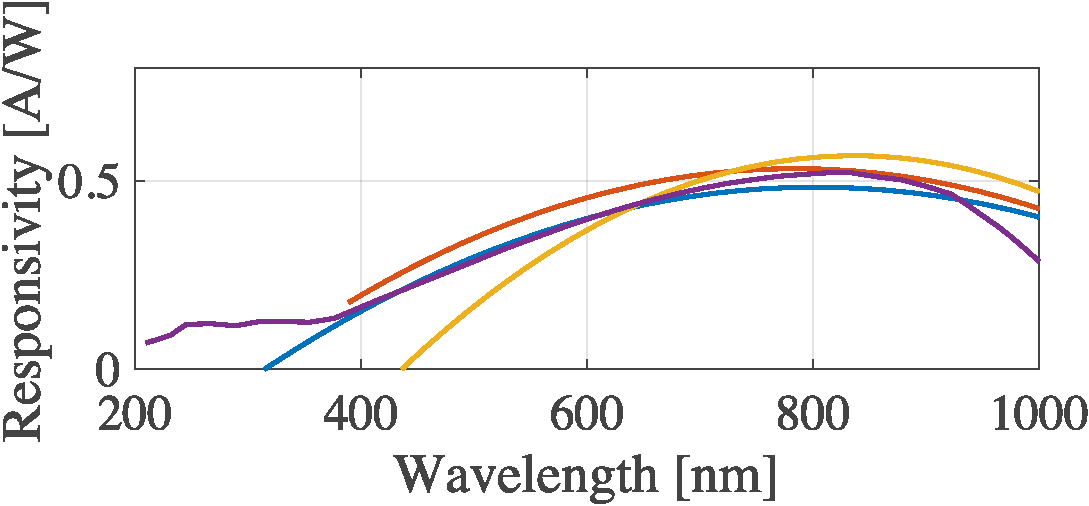
\includegraphics[width=0.5\columnwidth,draft=false]{./ch_background/figs/responsivity.pdf}
                \caption{Responsivities of four different Silicon-based \glspl{pd} taken from \protect\cite{edmundoptics}. (Please refer to \protect\cite{edmundoptics} for more detailed information on the corresponding curves. Note that details are removed for clarity purposes.)}
                \label{fig:ch_background:responsivity}
            \end{center}
        \end{figure}


    % In addition, as the downlink and uplink transmissions are assumed to occupy the \gls{vl} and \gls{ir} spectra, respectively, the comparisons of the \glspl{cir} over both spectra are worth discussing here.
    % Note that throughout this thesis, the wavelength range of 800 nm to 1,000 nm is considered when a signal is transmitter over the \gls{ir} spectrum.
    % The assumptions of the system model in this chaptesr are also used for that in the next chapters.   

    

\section{LiFi Channel Model}
\label{ch:ch_background:channelmodel}
    
% \subsection{Transmission Model}
% \label{ch:ch_background:transmissionmodel}
    
    
    Based on \cite{kahnkrause,infraredkahn}, the received optical power can be expressed as:
        \begin{align}
            y(t) = h(t) \circledast x(t),
        \end{align}
    where $\circledast$ denotes the convolution operation. 
    


\subsection{Channel Model}
\label{ch:ch_background:owcsimpy}

    
    For the sake of the illustrations, different opacities of faces in \figref{fig:ch_background:owcsimpy}(b) show different reflectivities, i.e., the head portions of the models have different reflectivities compared to the body portions of the model.
    

        \begin{figure}[h]
        \centering
        \begin{subfigure}[b]{0.49\columnwidth}
            \centering
            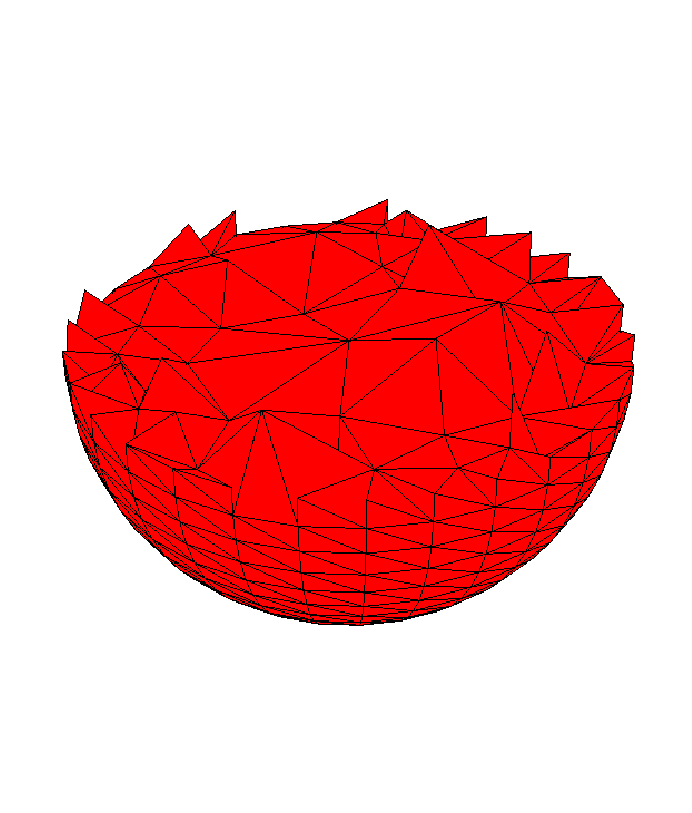
\includegraphics[width=0.5\columnwidth,draft=false]{./Appendix/figs/arb3d.pdf}
            \caption{}
        \end{subfigure}~
        \begin{subfigure}[b]{0.49\columnwidth}
            \centering
            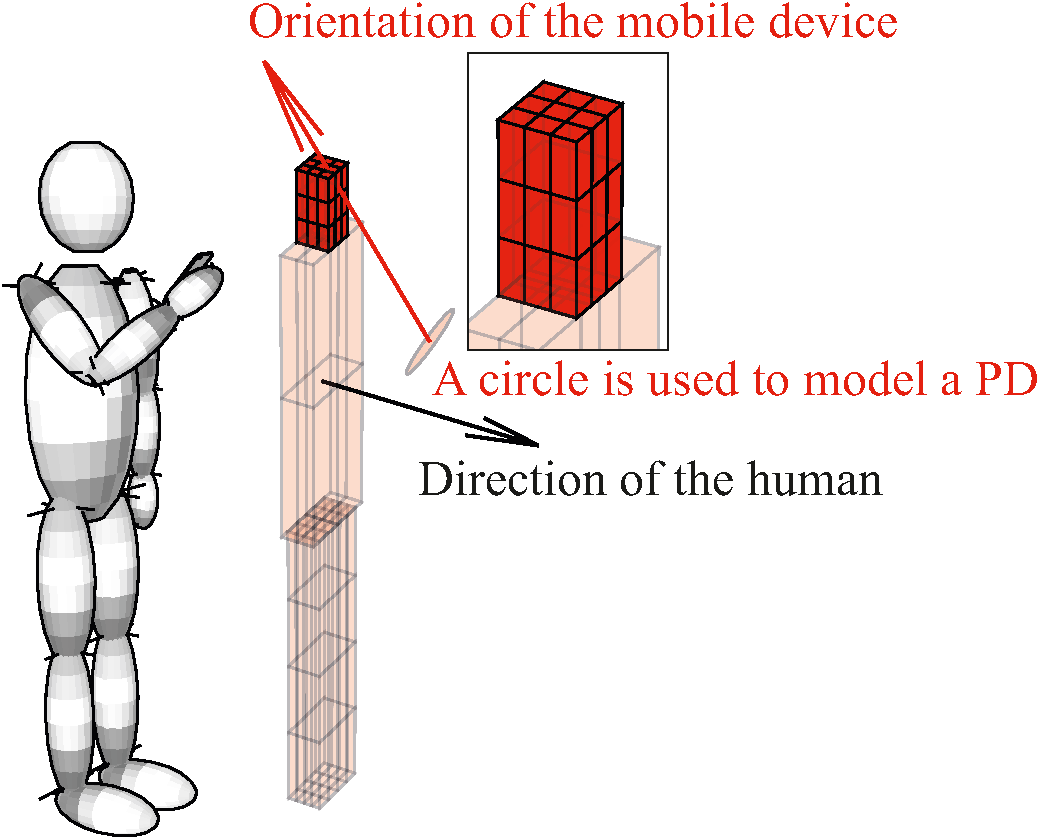
\includegraphics[width=0.85\columnwidth,draft=false]{./ch_background/figs/humanmodel_rev2.pdf}
            \caption{}
        \end{subfigure}
        \caption{(a) An example of a 3D object as a collection of 2D faces, and (b) a human model as a collection of square faces.}
        \label{fig:ch_background:owcsimpy}
      \end{figure}

    

\subsection{A Simple Office Environment}
\label{ch:ch_background:simpleoffice}

    
    
    

      \begin{table}[t]
        \caption{Reflectivities of materials over visible light (VL) and infrared (IR) spectrum.}
        \label{tab:reflectivity}
        \centering
        \begin{tabularx}{\columnwidth}{|l||Y|Y|Y|Y|c|}
        % \begin{tabular}{|l||c|c|c|c|c|}
        \hline
        Materials:               & paint & cotton & skin & plaster & pinewood \\ \hline
        Reflectivities (@ 940 nm): & 0.04               & 0.65   & 0.70 & 0.85    & 0.92 \\ \hline
        Reflectivities (@ 850 nm): & 0.04               & 0.64   & 0.66 & 0.83    & 0.92 \\ \hline  
        % \end{tabular}
        \end{tabularx}
      \end{table}

    Summaries of the reflectivities of the materials can be found in Table~\ref{tab:reflectivity}. 

    

         \begin{figure}[h]
            \centering
            \begin{subfigure}[b]{0.49\columnwidth}
                \centering
                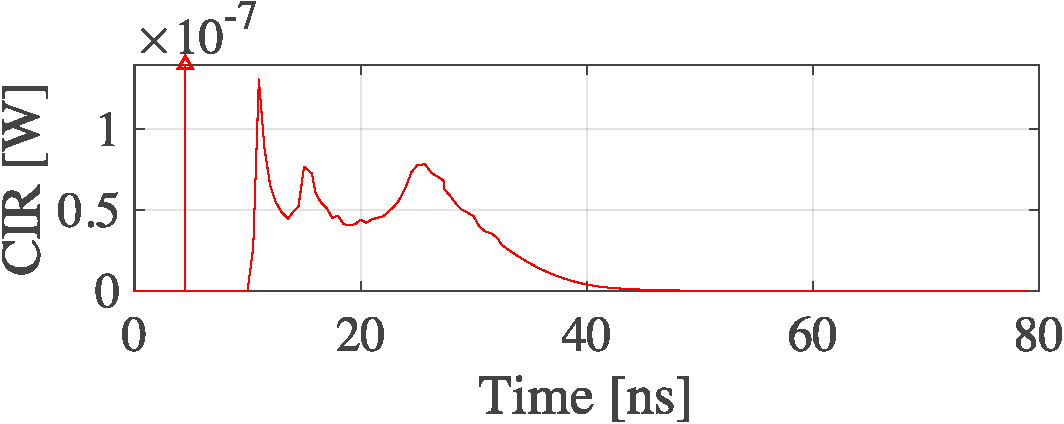
\includegraphics[width=1\columnwidth,draft=false]{./ch_background/figs/case1_ul_n.pdf}
                \caption{Case 1: 940 nm}
            \end{subfigure}~
            \begin{subfigure}[b]{0.49\columnwidth}
                \centering
                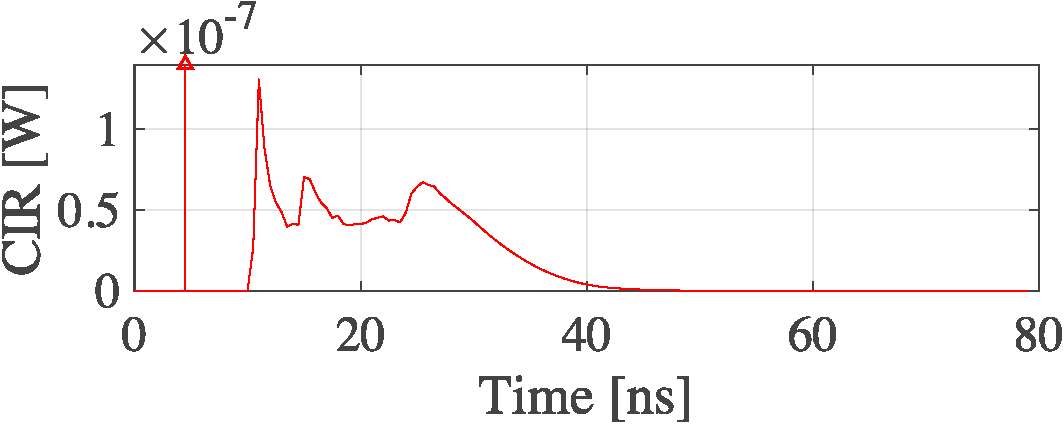
\includegraphics[width=1\columnwidth,draft=false]{./ch_background/figs/case1_ul.pdf}
                \caption{Case 1: 850 nm}
            \end{subfigure}\\
            \begin{subfigure}[b]{0.49\columnwidth}
                \centering
                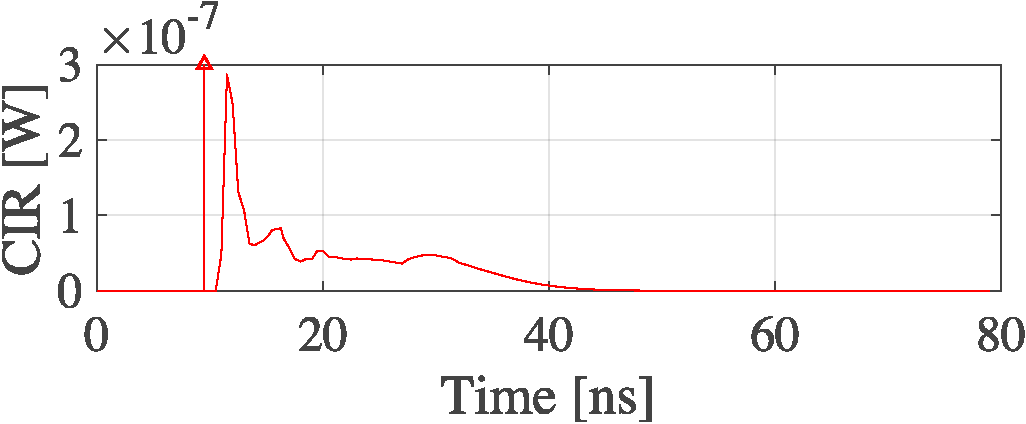
\includegraphics[width=1\columnwidth,draft=false]{./ch_background/figs/case2_ul_n.pdf}
                \caption{Case 2: 940 nm}
            \end{subfigure}~
            \begin{subfigure}[b]{0.49\columnwidth}
                \centering
                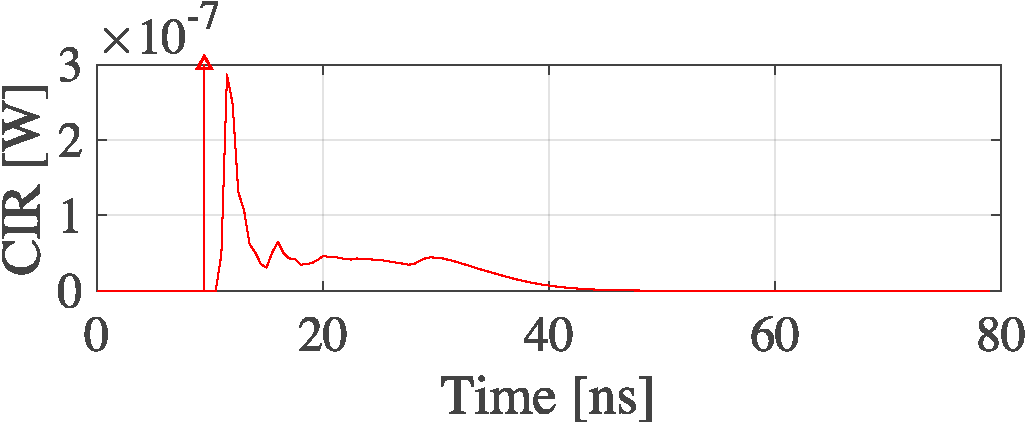
\includegraphics[width=1\columnwidth,draft=false]{./ch_background/figs/case2_ul.pdf}
                \caption{Case 2: 850 nm}
            \end{subfigure}\\
            \begin{subfigure}[b]{0.49\columnwidth}
                \centering
                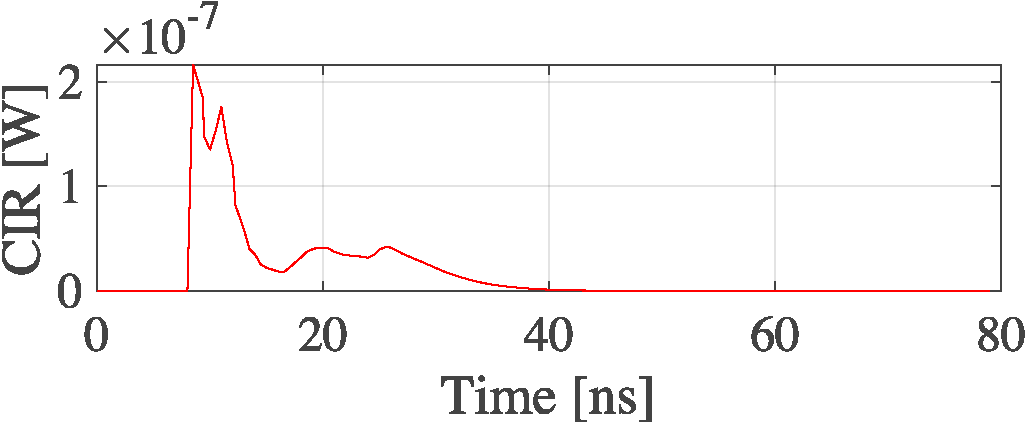
\includegraphics[width=1\columnwidth,draft=false]{./ch_background/figs/case3_ul_n.pdf}
                \caption{Case 3: 940 nm}
            \end{subfigure}~
            \begin{subfigure}[b]{0.49\columnwidth}
                \centering
                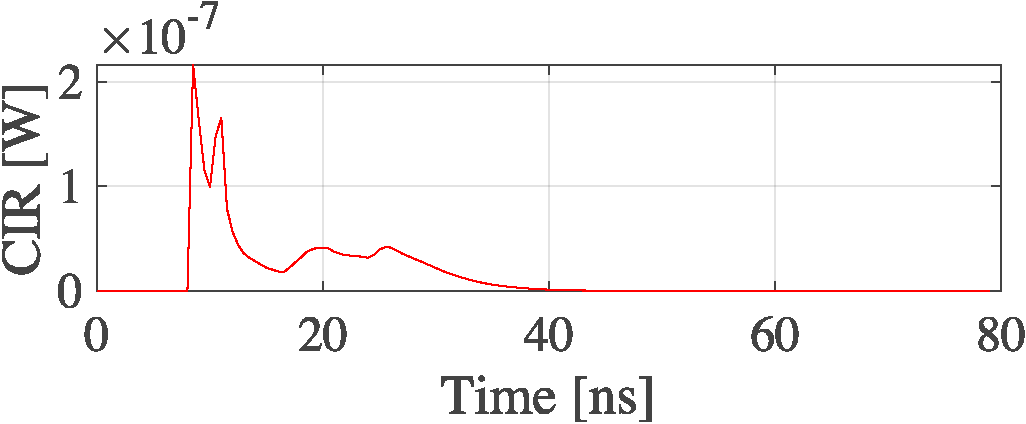
\includegraphics[width=1\columnwidth,draft=false]{./ch_background/figs/case3_ul.pdf}
                \caption{Case 3: 850 nm}
            \end{subfigure}
            \caption{CIRs.}
            \label{fig:ch_background:casesres}
        \end{figure} 




% \appendix indicates from now on \chapter generates an appendix
% rather than a normal chapter.
\appendix

\chapter{owcsimpy: A Library for Generating Wireless Optical CIRs}
\label{ch:app_owcsimpy}

\section{Introduction}

    \lipsum[2]

        \begin{figure}[h]
        \begin{lstlisting}[language=Python, caption=A Python snippet to generate a cuboid, label=lis:app_owcsimpy:cuboid]
cube = Cube(
    Vector(np.array([1,np.deg2rad(90),np.deg2rad(90)])),
    ctrPoint = np.array([0.5,0.5,0.5]),
    dimensions = [2,1,1],
    RodriguesAngle = np.deg2rad(30),
    reflectivities={'p0':0.5,'p1':0.5,'p2':0.5,
                    'p3':0.5,'p4':0.5,'p5':0.5}
)
planes = cube.getPartition(2)
fig,ax = draw(planes=planes,alphas=0.2,
    xlim=[-2,2],ylim=[-2,2],zlim=[-2,2],
    azim=-34,elev=9
 )
            \end{lstlisting}
        \end{figure}




% \let\cleardoublepage\clearpage

% \insertreferences inserts the list of references using the IEEE style
% and updates the table of contents. The single argument is a comma
% spearated list of .bib files (just as in \bibliography)
\insertreferences{References/thesis}
% \bibliographystyle{apalike}
% \bibliography{./References/thesis.bib}

% that's all folks!
\end{document}
